\let\negmedspace\undefined
\let\negthickspace\undefined
\documentclass[journal,12pt,twocolumn]{IEEEtran}

 \usepackage{gensymb}

 \usepackage{polynom}

\usepackage{amssymb}

\usepackage[cmex10]{amsmath}
\usepackage{amsthm}
\usepackage{graphicx}

 \usepackage{stfloats}

 \usepackage{bm}
\usepackage{longtable}

\usepackage{enumitem}
 

\DeclareMathOperator*{\Res}{Res}
\DeclareMathOperator*{\equals}{=}


\begin{document}

\bibliographystyle{IEEEtran}


\providecommand{\pr}[1]{\ensuremath{\Pr\left(#1\right)}}
\providecommand{\qfunc}[1]{\ensuremath{Q\left(#1\right)}}
\providecommand{\sbrak}[1]{\ensuremath{{}\left[#1\right]}}
\providecommand{\lsbrak}[1]{\ensuremath{{}\left[#1\right.}}
\providecommand{\rsbrak}[1]{\ensuremath{{}\left.#1\right]}}
\providecommand{\brak}[1]{\ensuremath{\left(#1\right)}}
\providecommand{\lbrak}[1]{\ensuremath{\left(#1\right.}}
\providecommand{\rbrak}[1]{\ensuremath{\left.#1\right)}}
\providecommand{\cbrak}[1]{\ensuremath{\left\{#1\right\}}}
\providecommand{\lcbrak}[1]{\ensuremath{\left\{#1\right.}}
\providecommand{\rcbrak}[1]{\ensuremath{\left.#1\right\}}}
\theoremstyle{remark}
\newtheorem{rem}{Remark}
\newcommand{\sgn}{\mathop{\mathrm{sgn}}}

\providecommand{\system}{\overset{\mathcal{H}}{ \longleftrightarrow}}
\newcommand{\question}{\noindent \textbf{Question: }}	
\newcommand{\solution}{\noindent \textbf{Solution: }}

\providecommand{\dec}[2]{\ensuremath{\overset{#1}{\underset{#2}{\gtrless}}}}

\vspace{3cm}
\title{I.C.S.E 12, 2019}

\author{ Burra Vishal Mathews\\CS21BTECH11010}
	


\maketitle
\question : 3(a) : If $x\bar=18$, $y\bar=100$, $\sigma_x=14$, $\sigma_y=20$ and correlation coefficient $r_{xy}=0.8$, find the regression equation of $y$ and $x$. 

\solution : \\
\textbf{Given : }$x\bar=18$, $y\bar=100$, $\sigma_x=14$, $\sigma_y=20$,$r_{xy}=0.8$\\
$$b_{yx}=r\times\frac{\sigma_y}{\sigma_x}=0.8\times\frac{20}{14}=\frac{8}{7}$$

The Regression equation y on x is :
\begin{equation}
    y-y\bar = b_{yx}(x-x\bar)\\
\end{equation}
\begin{align*}
    \implies&y-100=\frac{8}{7}(x-18)\\
    \implies&7y-700=8x-144\\
\end{align*}
\begin{equation}
    8x-7y+556=0
\end{equation}

$\therefore$ $8x-7y+556=0$ is the regression equation.

\begin{figure}[h!]
    \centering
    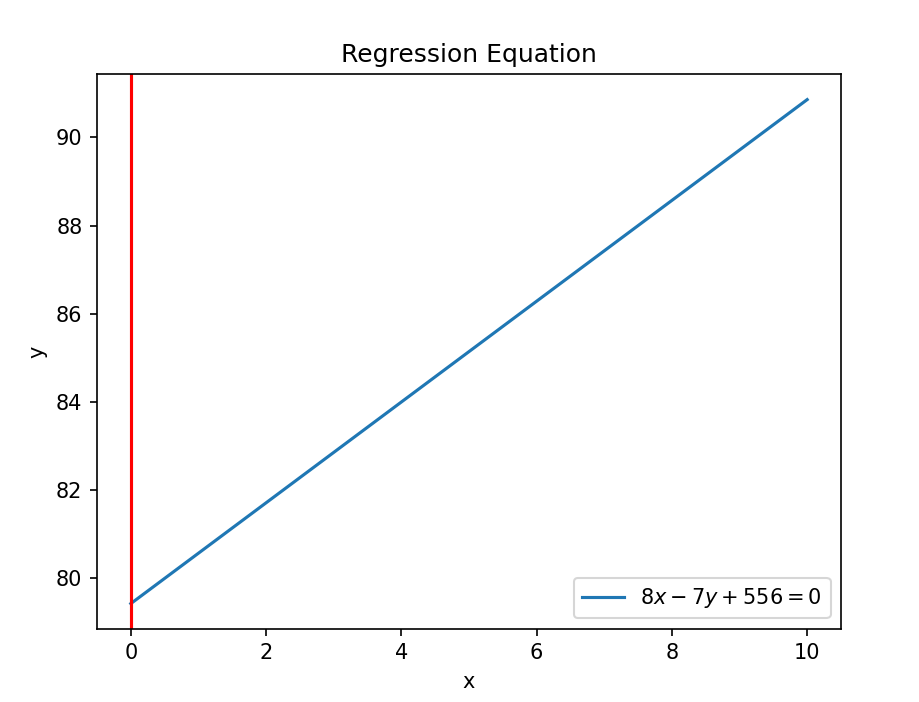
\includegraphics[width=\columnwidth]{figs/Asg2.png}
    \label{regeq}
\end{figure}
\end{document}